\subsection{Possible Explanations for Gender Differences}

\textbf{[JJH: Way too much emphasis on CBA.]}

These results and estimates of IRR/CBA \citep{Garcia_Heckman_Leaf_etal_2017_Comp_CBA_Unpublished} show gender differences. In this section, we discuss some of the mechanisms contributing to these differences and connect the results of the two papers.

On a superficial level, there is tension between the results in this paper favoring females and the results in \citet{Garcia_Heckman_Leaf_etal_2017_Comp_CBA_Unpublished} favoring males. There are two mutually inclusive explanations for this. One explanation is that although a larger proportion of the treatment effects are positive for females, those that are positive for males correspond to outcomes that can be monetized. For example, there is a strong treatment effect on labor income at age 30 for males, but not for females. When this income is projected over the life cycle in \citet{Garcia_Heckman_Leaf_etal_2017_Comp_CBA_Unpublished}, the males continue to benefit more from treatment than do females. In a related case, there are also outcomes that cannot be monetized for which treatment more positively impacts for females than for males. An example of this are variables related to family structure, such as number of children.

Another explanation for the higher benefit/cost ratio and internal rate of return for males is that even if there are treatment effects for both genders, a general characteristic of males in society can change the expression of that effect. An example of this is seen in crime. ABC/CARE positively and significantly reduced crime for both males and females. However, on average, males commit more crimes that have higher social costs (e.g. violent crimes) compared with females. Figure~\ref{fig:crime-tes-detail} illustrates this. Although ABC/CARE reduces criminal activity both of misdemeanors and felonies, the mean number of misdemeanors committed by the control-group females is very close to the analogous mean of the control-group males. This is not the case for felonies, which tend to be more serious (and costly) crimes.\footnote{This is also supported by \citet{Cohen-Bowles_2010_Estimating-Cost-Crime,Gregg_etal_2015_SocialRealities_BOOK,UDOJ_2016_PrisonersStatistics_Bulletin}.}

\begin{figure}[!htbp]
\centering
\caption{Treatment Effects on Crime, by Crime Type}
\label{fig:crime-tes-detail}
\begin{subfigure}[h]{0.5\textwidth}
	\centering
	\caption{Misdemeanors}
	\label{fig:crime-misdemeanors}
	\includegraphics[width=\textwidth]{output/bar-gender-trt-ad34_mis}
\end{subfigure}%
\begin{subfigure}[h]{0.5\textwidth}
	\centering
	\caption{Felonies}
	\label{fig:crime-felonies}
	\includegraphics[width=\textwidth]{output/bar-gender-trt-ad34_fel}
\end{subfigure}
\footnotesize \justify
Note: These plots show the mean misdemeanors and felonies of the treatment and control group by gender. The capped lines indicate standard errors and the points represent significant differences between treatment and control within each gender. These are estimated using 100 bootstraps. Both of these measures come from the administrative crime data collected when the subjects were approximately age 35.
\end{figure}

There is another important factor at play that is present in the results of both papers: the issue of alternative preschool. There are substantial differences between males and females in one counterfactual: treatment vs. alternative preschools. The estimated treatment effects are very similar across genders for treatment compared to those staying at home full time. Males benefit much more from treatment relative to alternative preschools compared to their benefits from treatment relative to staying at home. This result is consistent with findings noted elsewhere: (i) stark gender differences resulting from attending low quality childcare \citep{Kottelenberg-Lehrer_2014_Gender-Effects,Baker_Gruber_Milligan_2015_Noncog_Defects}; and (ii) females are less sensitive to uncertain environments (see, e.g., \citealp{Autor-etal_2015_Family-Disadvantage}).

In addition to a gender difference in alternative preschool experiences, there are gender differences in the experience of ABC/CARE treatment. We explore this by looking at the specific effects of the intervention on parenting.\footnote{In this exercise, we use We use measurements of the Home Observation for Measurement of the Environment (HOME; \citet{Bradley-Caldwell_1977_AJMD}). Although the exact scales vary by age, the subscales of the HOME measure generally measure maternal warmth and involvement, absence of punishment, provision of appropriate toys, encouragement of mature behavior and independence, and the physical and language environment. The full score is the sum of these subscales.}

When graphing the density of a factor combining the parenting skills measured at different ages, the density of the treatment group in both the male and female subsamples is bimodal (Figure~\ref{fig:total-home}). Because this is not the case for the control group, it is possible that treatment is moderated by another input of home environment. We consider the input of father's presence because it is highly correlated with selection into alternative preschool. For males, the mean of the treatment group if the father is present is greater than that of the treatment group if the father is absent. The reverse is seen for the females.

\begin{figure}
\begin{center}
\caption{Density of the HOME Scores by Gender and Experimental Group}
\label{fig:total-home}

	\begin{subfigure}[b]{0.49\textwidth}
		\centering
		\caption{Parenting Skills, Males}
		\label{fig:home-male-factor}
			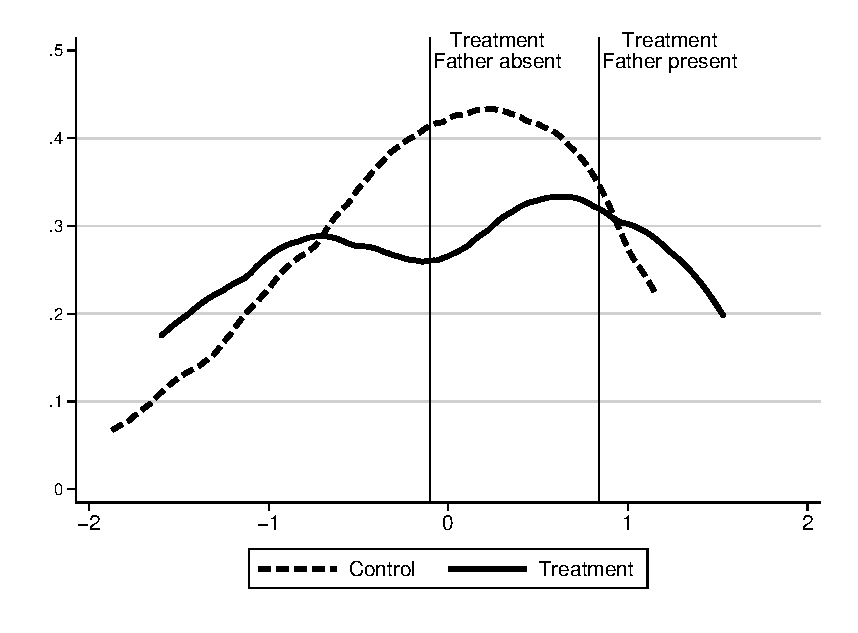
\includegraphics[width=\textwidth]{output/HOME-males-factorhome}
	\end{subfigure}
	\begin{subfigure}[b]{0.49\textwidth}
		\centering
		\caption{Parenting Skills, Females}
		\label{fig:home-female-factor}
			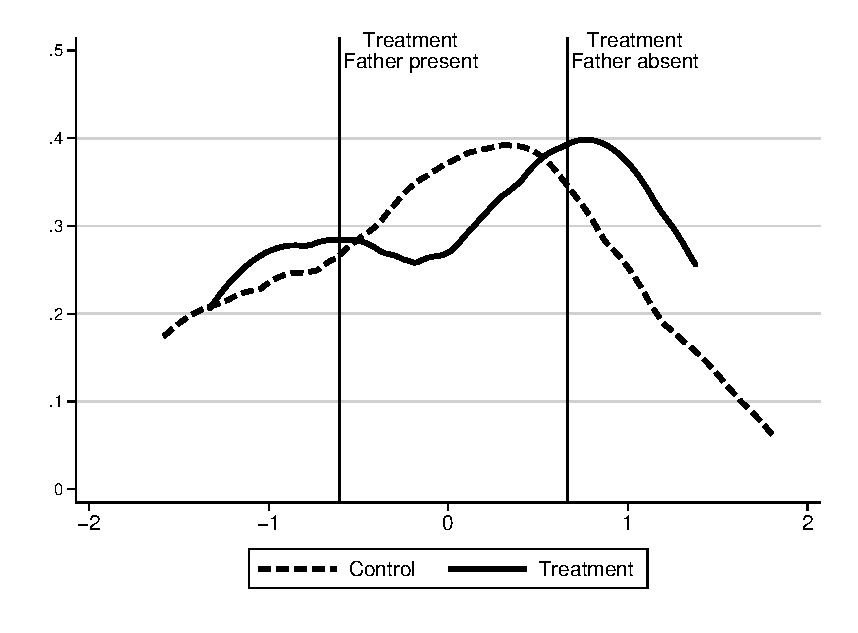
\includegraphics[width=\textwidth]{output/HOME-females-factorhome}
	\end{subfigure}
\end{center}
\raggedright
Note: These plots show the distribution the factor of HOME scores. The factors are computed by gender using full HOME scores at 0.5, 1.5, 2.5, and 8 years. The vertical lines are the means of the treatment group by father's presence.
\end{figure}

We explore this trend more closely in Figure~\ref{fig:total-home-quantiles}. To do so, we calculate the distribution pooling experimental groups but splitting by gender and father's presence. We then calculate, by gender and father's presence, the proportion of the treatment group that is in quantile 1 versus quantile 2. We do the same for the control group.

\begin{sidewaysfigure}
\begin{center}
\caption{Factor HOME Scores}
\label{fig:total-home-quantiles}
	\begin{subfigure}[b]{0.49\textwidth}
		\centering
		\caption{HOME, Father Absent, Males}
		\label{fig:home-male-mean}
			\includegraphics[width=\textwidth]{output/HOME-male1-fhome0-2quant}
	\end{subfigure}
	\begin{subfigure}[b]{0.49\textwidth}
		\centering
		\caption{HOME, Father Absent, Females}
		\label{fig:home-female-mean}
			\includegraphics[width=\textwidth]{output/HOME-male0-fhome0-2quant}
	\end{subfigure}
	
	\begin{subfigure}[b]{0.49\textwidth}
		\centering
		\caption{HOME, Father Present, Males}
		\label{fig:home-male-factor}
			\includegraphics[width=\textwidth]{output/HOME-male1-fhome1-2quant}
	\end{subfigure}
	\begin{subfigure}[b]{0.49\textwidth}
		\centering
		\caption{HOME, Father Present, Females}
		\label{fig:home-female-factor}
			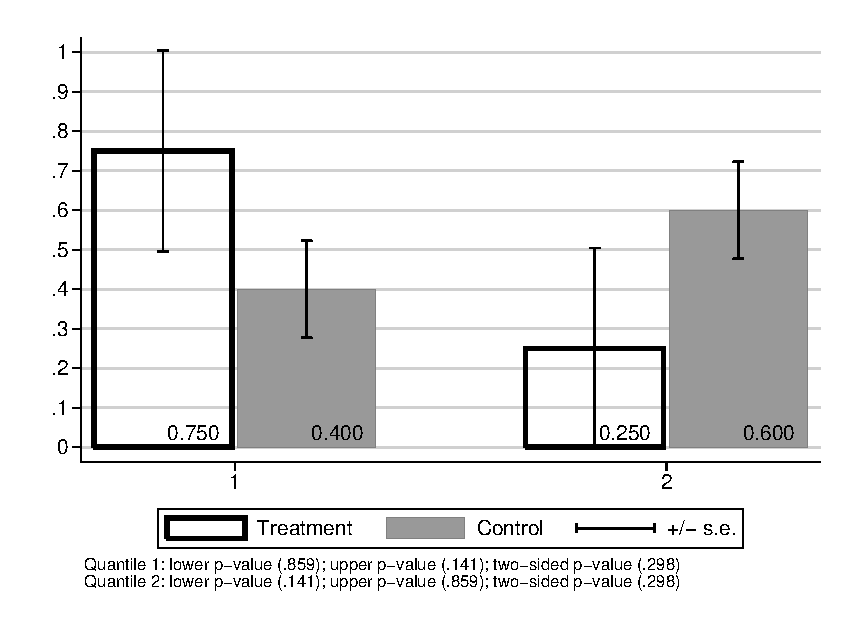
\includegraphics[width=\textwidth]{output/HOME-male0-fhome1-2quant}
	\end{subfigure}
\end{center}
\raggedright \footnotesize
Note: The horizontal axis divides a factor of the HOME scores into the first and second quantile of the distribution pooling across experimental groups, but splitting  by gender and father's presence. The factors are computed by gender using full HOME scores at 0.5, 1.5, 2.5, and 8 years. The lower $p$-value tests that the treatment proportion is less than the control proportion within a quantile. The upper $p$-value tests that the treatment proportion is greater than the control proportion within a quantile. The numbers reported in the bars are the proportions. All standard errors and $p$-values are calculated using 1,000 bootstraps.
\end{sidewaysfigure}

The result of this exercise shows that the bimodal shape of the densities of the treatment group is explained differently by gender. For males, the parenting measures are higher for the control group when the fathers are absent and higher for the treatment group when father's are present. For females, the opposite is the case: The parenting measures are higher for the control group when fathers are present and higher for the treatment group when fathers are absent.

This example illustrates that treatment complements father's presence for males but substitutes it for females. That is, treatment compensates for early life disadvantage for males, but substitutes it for females. This explains how early-life skill differences favoring females can still translate to later-life outcomes favoring males. Although males initially face deficits, the program compensates for these deficits helping them catch up to females. Additional factors in the larger economy can then widen differences later in life when the subjects enter the labor market.

\textbf{[JJH: Report results for controls (see comment 7a \& 7b). We need to deemphasize CBA. We are spoiling its market.]}


